

\underline{i quiz non hanno penalità e non c'è minimo}
seconda parte con 17 punti

\section{Sistema dinamico}
\begin{tcolorbox}[colback=yellow!10, colframe=black]
Un sistema dinamico è un oggetto matematico adatto a descrivere qualsiasi fenomeno ``fisico'', in particolare questo formalismo matematico può essere utilizzato per studiare il comportamento di qualsiasi fenomeno con l'obiettivo di analizzare, simulare, predirre e \underline{controllare} le variazioni nel tempo delle grandezze che caratterizzano il fenomeno oggetto dello studio.
\end{tcolorbox}
\begin{center}
    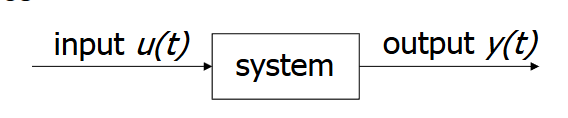
\includegraphics[width=0.5\textwidth]{foto/cph1/1.png}
\end{center}
Un esempio che possiamo fare è un esempio meccanico di uno spostamento di un blocco soggetto ad attrito a cui applichiamo una certa forza.
Vogliamo studiare il comportamento della massa al variare della forza.
\begin{itemize}
    \item Ingresso: $u(t)=F(t)$
    \item Uscita: $y(t)= p(t)$
    \item Soluzione: $F(t) - \beta \cdot v(t) = m\cdot a(t) \rightarrow F(t) - \beta \cdot \dot{p}(t) = m\cdot \ddot{p}(t)$
\end{itemize}
La soluzione quindi risulta essere l'equazione differenziale che descrive matematicamente la relazione quantitativa tra ingresso e uscita.
La determinazione di questa relazione è l'obiettivo principale dello studio dei sistemi dinamici.
\subsection{Differenze tra sistema statico e sistema dinamico}
Procediamo per esempi:
\begin{itemize}
    \item Vogliamo studiare la caduta di tensione ai capi di un resistore di un circuito semplice a cui basta applicare la legge di Ohm.
            \begin{itemize}
            \item Ingressi: $u(t) = i(t)$
            \item Uscite: $y(t) = V(t)$
            \item Soluzione: $V(t) = R \cdot i(t)$
            \begin{tcolorbox}[colback=yellow!10, colframe=black]
                Un sistema si dice statico se il valore della sua uscita in un certo istante di tempo t dipende solo dal valore degli ingressi nello stesso istante di tempo t.
            \end{tcolorbox}
        \end{itemize} 
    \item Vogliamo studiare la caduta di tensione ai capi di un condensatore a cui basta applicare la legge di Ohm.
            \begin{itemize}
            \item Ingressi: $u(t) = i(t)$
            \item Uscite: $y(t) = V(t)$
            \item Soluzione: $V(t) = \frac{1}{C} \int_{-\infty}^{t} u(t) dt$
            \item Se vogliamo esprimere la soluzione in forma differenziale, possiamo derivare entrambi i membri dell'equazione e otteniamo $\dot{y}(t) = \frac{1}{C} \cdot u(t)$
            \begin{tcolorbox}[colback=yellow!10, colframe=black]
                Un sistema si dice dinamico se il valore della sua uscita in un certo istante di tempo t dipende dai valori degli ingressi in istanti di tempo precedenti a t.
            \end{tcolorbox}
        \end{itemize}   
\end{itemize}
\newpage
Considerazioni che possiamo fare:
\begin{itemize}
    \item Un sistema dinamico è un sistema che ha memoria, ovvero il suo comportamento dipende da ciò che è accaduto in passato.
    \item Un sistema statico è un sistema che non ha memoria, ovvero il suo comportamento dipende solo da ciò che accade nel presente, quindi caso particolare di un sistema dinamico.
    \item Riconosco un sistema dinamico se è possibile descrivere il suo comoprtamento con un'equazione differenziale, altrimenti è un sistema statico.
\end{itemize}
\subsection{Descrizione dei sistemi dinamici mediante le equazioni di ingresso-stato-uscita (descrizione matematica nello spazio di stato $\leftrightarrow$ state-space description)}
Possiamo aggirare il problema della mancanza di memoria dei sistemi dinamici, introducendo delle variabili ausiliarie che ci permettono di tenere traccia di ciò che è accaduto in passato. Ipotizziamo che dobbiamo calcolare gli ingressi che vanno da $t_0$ a $t$, se introduciamo una variabile ausiliaria $x(t)$.
Se prendo in esame l'esempio del condensatore:
\begin{itemize}
    \item Ingresso: $u(t) = i(t)$
    \item Uscita: $y(t) = V(t)$
    \item Soluzione: $y(t) = \frac{1}{C} \int_{-\infty}^{t} u(t) dt$
    \item Introduciamo la variabile ausiliaria $y(t_0)= x(t) = \int_{-\infty}^{t_0} u(t) dt$, quindi $y(t) = x(t) + \frac{1}{C} \int_{t_0}^{t} u(t) dt$
\end{itemize}
Il mio stato corrente del sistema, quindi prima degli ingressi che mi interessano, è dato da $x(t) = y(t_0)$, che rappresenta la memoria del sistema, ovvero ciò che è accaduto in passato, e da $u(t)$, che rappresenta ciò che sta accadendo nel presente.
\begin{tcolorbox}[colback=yellow!10, colframe=black]
    Ogni sistema dinamico a tempo continuo può essere descritto matematicamente nel seguente modo:
    \[
    \begin{cases}
        \dot{x}(t) = f(x(t), u(t), t) \\
        y(t) = g(x(t), u(t), t)
    \end{cases}
    \]
    Queste equazioni sono dette equazioni di ingresso-stato-uscita, dove $x(t)$ è lo stato del sistema, $u(t)$ è l'ingresso del sistema e $y(t)$ è l'uscita del sistema.
\end{tcolorbox}
Se torniamo all'esempio del condensatore, possiamo scrivere le equazioni di ingresso-stato-uscita nel seguente modo:
\[
\begin{cases}
    \dot{x}(t) = \frac{1}{C}u(t) \\
    y(t) = x(t)
\end{cases}
\]
Se invece consideriamo l'esempio del blocco soggetto ad attrito, possiamo scrivere le equazioni di ingresso-stato-uscita nel seguente modo, che era definita in precedenza come equazione differenziale $F(t) - \beta \cdot \dot{p}(t) = m\cdot \ddot{p}(t)$:
\[
\begin{cases}
    V(t) =\dot{p}(t) \\
    a(t) = \dot{V}(t) = \ddot{p}(t)
\end{cases}
\]
Da cui otteniamo:
\[
\begin{cases}
    F(t)-\beta \cdot V(t) = m \cdot a(t) \\
    V(t) = \dot{p}(t)
\end{cases}\]
Ed infine otteniamo che le equazioni di ingresso-stato-uscita sono:
\[
\begin{cases}
    \dot{x}_1(t) = x_2(t) \\
    \dot{x}_2(t) = \frac{1}{m}u(t) - \frac{\beta}{m}x_2(t) \\
    y(t) = x_1(t)
\end{cases}
\]
Quindi lo stato di spazio è dato da $x(t) = \begin{bmatrix} x_1(t)=p(t) \\ x_2(t)=V(t) \end{bmatrix}$, l'ingresso è dato da $u(t) = F(t)$ e l'uscita è data da $y(t) = p(t)$.
\section{Sistema di controllo}
\subsection{Componenti di un sistema di controllo}
Un sistema di controllo è composto da:
\begin{itemize}
    \item Un sistema da controllare, chiamato \textit{plant} (sistema oggetto del controllo)
    \item Un \textit{controller} (sistema che genera il segnale di controllo)
    \item Un \textit{sensore} (sistema che misura l'uscita del sistema da controllare)
    \item Un elemento di riferimento (sistema che fornisce il segnale desiderato)
\end{itemize}
\begin{center}
    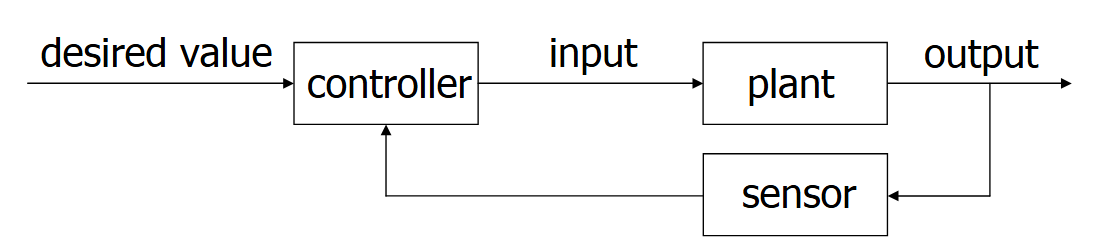
\includegraphics[width=0.5\textwidth]{foto/cph1/2.png}
\end{center}
